\documentclass[final]{beamer}
\usepackage{grffile}
\mode<presentation>
\usetheme{le2i}
\usepackage[utf8]{inputenc}
\usepackage[english]{babel}
\usepackage{amsmath,amsthm, amssymb, latexsym}
\usepackage{enumitem}
\usepackage{multirow}
\usepackage[single=true, macros=true, xspace=true]{acro}
\usepackage{algorithm}
\usepackage{algpseudocode}
\usepackage{cleveref}
\usepackage{ragged2e}
\usepackage{latexsym}
\usepackage{xcolor}
\usepackage{epsf,graphicx,subfig}
\usepackage{epstopdf}
\usepackage{subfig}	
%% In order to draw some graphs
\usepackage{tikz,xifthen}
\usetikzlibrary{decorations.pathmorphing}
\usetikzlibrary{fit}
\usetikzlibrary{backgrounds}
\usetikzlibrary{shapes,arrows,shadows}
\usetikzlibrary{calc,decorations.pathreplacing,decorations.markings,positioning}
\usetikzlibrary{snakes,decorations.text,shapes,patterns}

\boldmath
\usepackage[orientation=portrait,size=a0,scale=1.4,debug]{beamerposter}
\usepackage{array,booktabs,tabularx}
\newcolumntype{Z}{>{\centering\arraybackslash}X} % centered tabularx columns
\newcommand{\pphantom}{\textcolor{ta3aluminium}} % phantom introduces a vertical space in p formatted table columns??!!

\setbeamertemplate{bibliography item}[text]

\newcolumntype{L}{>{\arraybackslash}m{22cm}}
\newcolumntype{S}{>{\arraybackslash}m{5cm}}

%%%%%%%%%%%%%%%%%%%%%%%%%%%%%%%%%%%%%%%%%%%%%%%%%%%%%%%%%%%%%%%%%%%%%%%%%%%%%%%%%%%%%%
\title{\huge Reflectance Confocal Microscopy and Lentigo: Evaluation of several feature extractors for automatic detection}

\author{Romain Cendre\inst{1}, Alamin Mansouri\inst{1}, Jean-Luc Perrot\inst{2}, Elisa Cinotti\inst{3}, Franck Marzani\inst{1} }

\institute{ \inst{1} Laboratoire ImViA EA 7535, Université de Bourgogne, Dijon, France\\
            \inst{2} Service de Dermatologie-Oncologie-Allergologie, CHU de St Etienne, France\\
            \inst{3} U.O. Dermatologia, Dipartimento di Scienze Mediche, Università degli Studi di Siena, Italy}
\date{March. 14th 2019}

%%%%%%%%%%%%%%%%%%%%%%%%%%%%%%%%%%%%%%%%%%%%%%%%%%%%%%%%%%%%%%%%%%%%%%%%%%%%%%%%%%%%%%
\newlength{\columnheight}
\setlength{\columnheight}{80cm}
%% Acronym definition example using glossaries package
%% \usepackage{acro} is required
%% 
%% For a powerful usage of the acro package look at http://tex.stackexchange.com/questions/135975/how-to-define-an-acronym-by-using-other-acronym-and-print-the-abbreviations-toge

\DeclareAcronym{cnn}{
  short = CNN,
  long = Convolutional Neural Network
}

\DeclareAcronym{pca}{
  short = PCA,
  long = Principal Component Analysis
}

\DeclareAcronym{rcm}{
  short = RCM,
  long = Reflectance Confocal Microscopy
}

\DeclareAcronym{roc}{
  short = ROC,
  long = Receiver Operating Characteristic
}

 

%%%%%%%%%%%%%%%%%%%%%%%%%%%%%%%%%%%%%%%%%%%%%%%%%%%%%%%%%%%%%%%%%%%%%%%%%%%%%%%%%%%%%%
\begin{document}

\begin{frame}
  \begin{columns}[t]
    %----------------------------------------------------------%
    %             		FIRST COLUMN 						  %
	%----------------------------------------------------------%
    \begin{column}{.49\textwidth}
      \begin{beamercolorbox}[center,wd=\textwidth]{postercolumn}
        \begin{minipage}[T]{.95\textwidth}  % tweaks the width, makes a new \textwidth
          \parbox[t][\columnheight]{\textwidth}{
            % fill each column with content     
            \begin{block}{Introduction}
                \justifying
               Skin cancer is considered as one of the most important pathologies of these days, having a daily impact on affected people and strong economic consequences over the world. An early detection can help to prevent most of the repercussions. Many imaging tools have been designed to prevent skin pathologies. For that purpose, this work focuses on \ac{rcm} images for automated diagnosis of Lentigo, a specific type of skin pathology.
               
        	    \begin{figure}
                    \includegraphics[width=.9\linewidth]{content/figures/Data.png}
				\end{figure}
            \end{block}   
            \vspace{0.1in}
            \begin{block}{Methods}
                This paper evaluates three feature extractors:
                \hspace*{2.5cm}
                    \begin{tabular*}{0.8\textwidth}{rll}
                          \textbf a) & \(\text{Wavelets \cite{Halimi2017a}}\)  & \(\rightarrow \text{Based on Daubechies.}\) \\
                          \textbf b) & \(\text{Haralick \cite{Haralick1973}}\) & \(\rightarrow \text{Using four directions.}\) \\
                          \textbf c) & \(\text{Deep Features \cite{Litjens2017}}\) & \(\rightarrow \text{Using InceptionV3 architecture.}\) \\
                    \end{tabular*}
				\begin{figure}[h]
                \centering
                  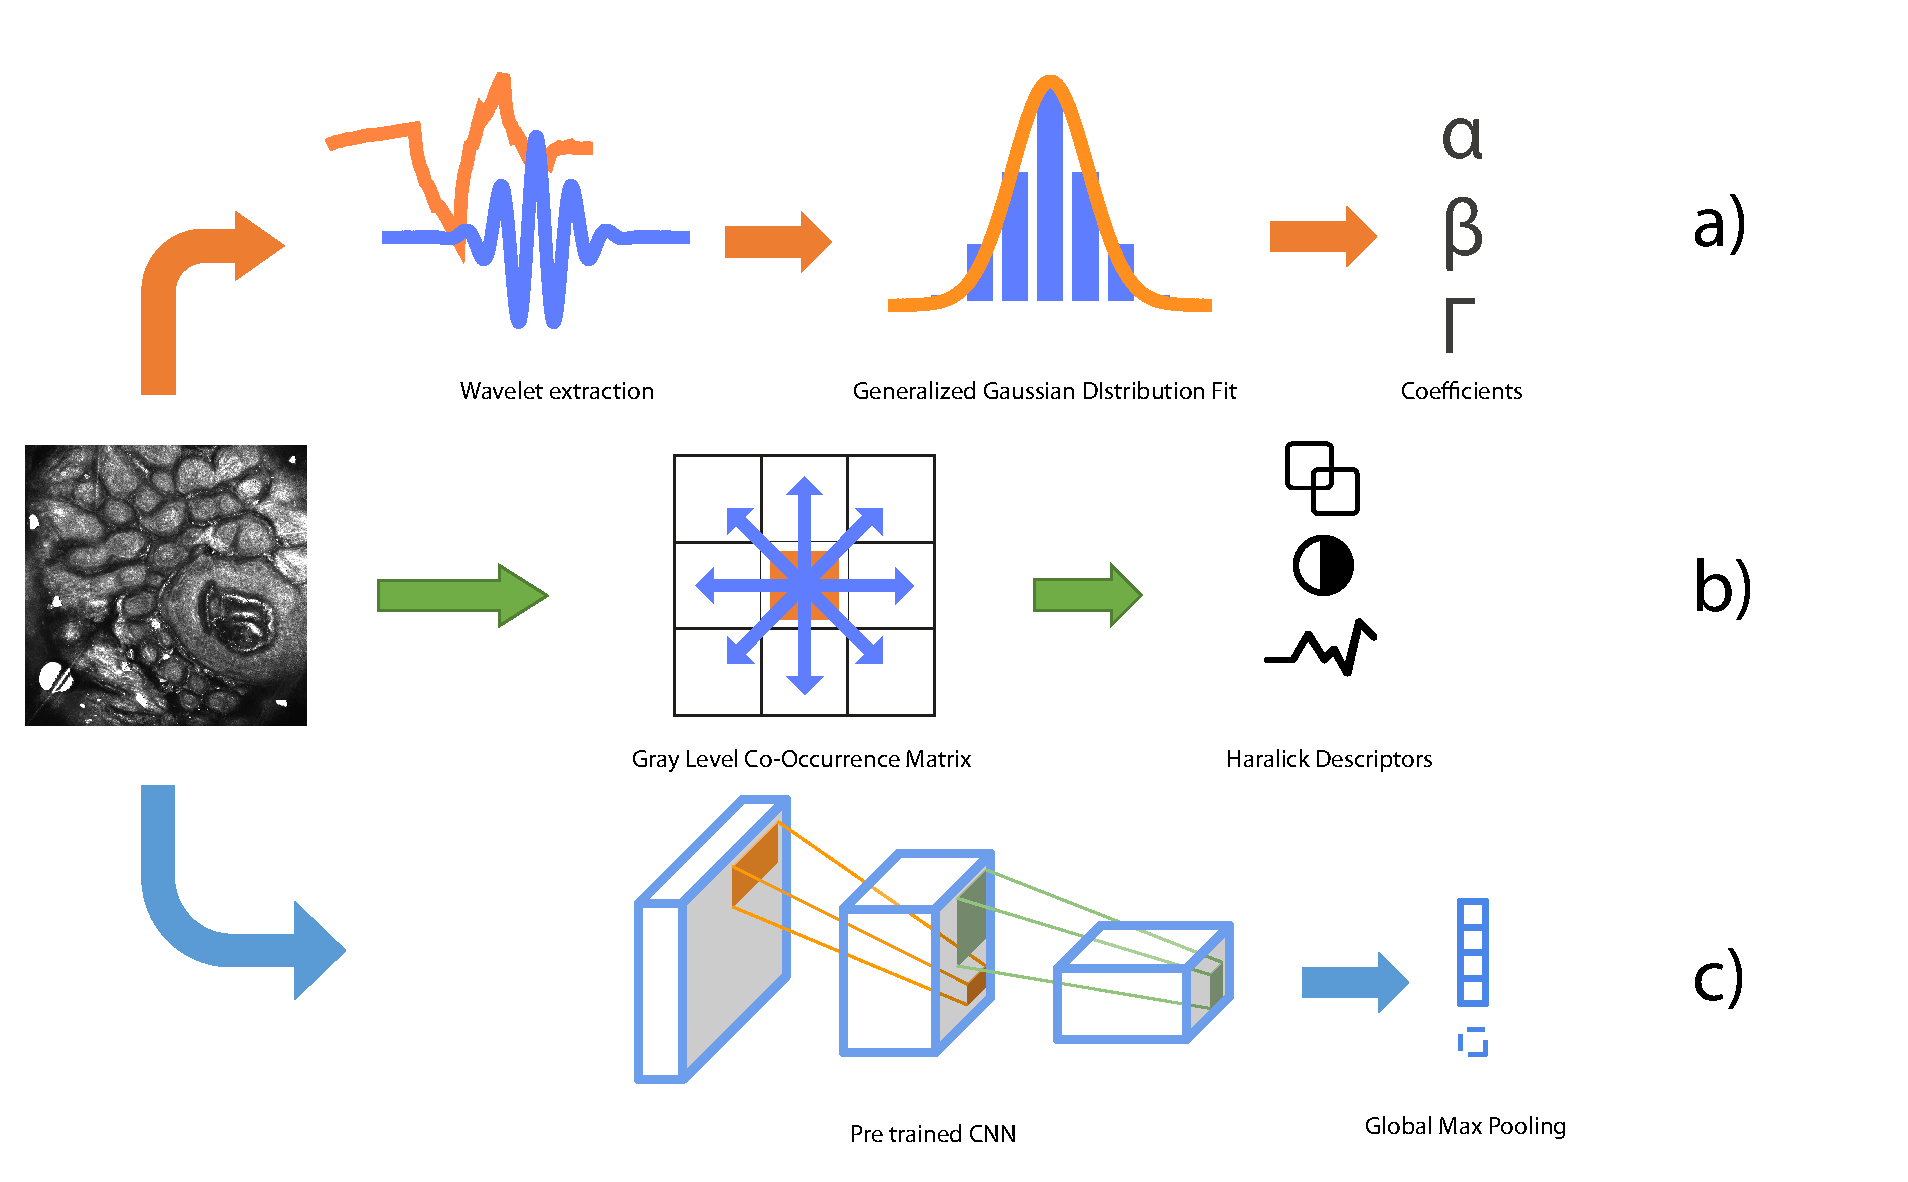
\includegraphics[width=\linewidth]{content/figures/Methods.pdf}
                  \label{fig:method_used}
                \end{figure}
                All of these feature extractors are evaluated using a machine learning pipe. First, features are normalized using a standard score computation. Then, a classification task is performed by a classical SVM using linear kernel.\par
                \begin{figure}[h]
                \centering
                  \includegraphics[width=.9\linewidth]{content/figures/Process.pdf}
                  \label{fig:pipeline}
                \end{figure}
            \end{block}       
           }
        \end{minipage}
      \end{beamercolorbox}
    \end{column}
    % ---------------------------------------------------------%
    % end the column
    
    %----------------------------------------------------------%
    %             		SECOND COLUMN 						  %
	%----------------------------------------------------------%
	\begin{column}{.49\textwidth}
	\begin{beamercolorbox}[center,wd=\textwidth]{postercolumn}
        \begin{minipage}[T]{.95\textwidth}  % tweaks the width, makes a new \textwidth
          \parbox[t][\columnheight]{\textwidth}{ % must be some better way to set the the height, width and textwidth simultaneously
            \begin{block}{Results}
                \justifying
                The evaluation of descriptors uses three metrics: Precision, Recall and F1-Score.
                Our validation protocol takes advantage of nested cross validation, more robust than simple cross validation \cite{Cawley2010}. Table below shows that Haralick and Deep Features perform well and are more robust for classification task than Wavelets based approach.
                \begin{table}[h]
                    \centering
                    \begin{tabular*}{\textwidth}{l@{\extracolsep{\fill}}lll}
                        \hline
                        Methods & Precision & Recall & F1-Score \\
                        \hline
                        Wavelets & 0.69$\pm$0.04 & 0.69$\pm$0.04 & 0.68$\pm$0.05 \\
                        \hline
                        Haralick & 0.84$\pm$0.02 & 0.83$\pm$0.02 & 0.83$\pm$0.02 \\
                        \hline
                        Deep Features & 0.89$\pm$0.02 & 0.89$\pm$0.02 & 0.89$\pm$0.02 \\
                        \hline
                    \end{tabular*}
                    \label{table:averages}
                \end{table}
                These results are correlated to PCA projection on two first dimensions, shown in next Figure.
                \begin{figure}                                    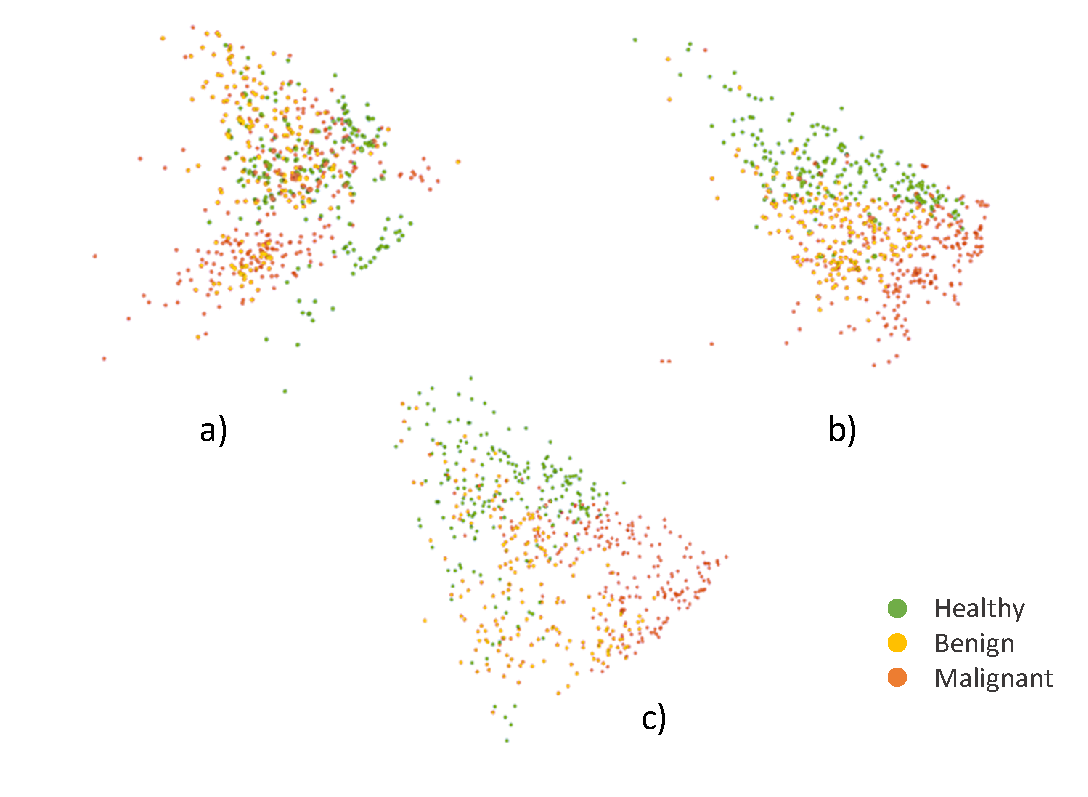
\includegraphics[width=0.7\linewidth]{content/figures/Projection.pdf}
				\end{figure}
                A focus on Deep Features ROC curves shows that features provided are relevant for "Healthy" prediction, compared to "Benign" and "Malignant" classes.
                \begin{figure}
                    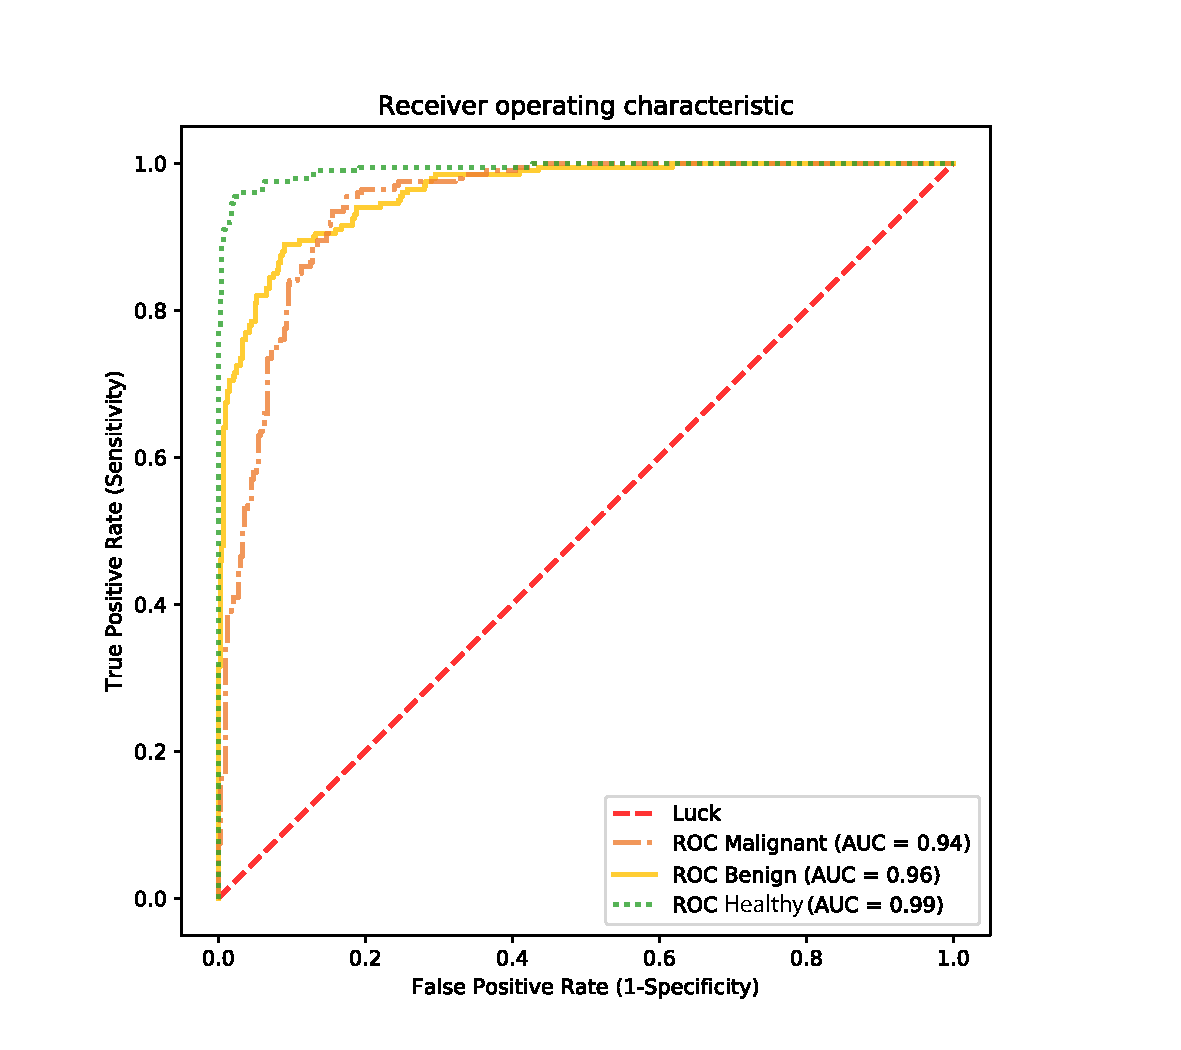
\includegraphics[width=0.65\linewidth]{content/figures/ROC.pdf}
				\end{figure}
            \end{block}
            \vspace{0.1in}
            \begin{block}{Conclusion and Future Work}
            \justifying
              Pertinence of three extraction methods on \ac{rcm} images for diagnosis of Lentigo were evaluated on this study. Haralick and Deep Features approaches shown the most relevant results on classification of patches based on three classes. In further work we will classify whole images using a patch decomposition method or using a Deep Learning end-to-end solution.
            \end{block}
            }
        \end{minipage}
    \end{beamercolorbox}    
	\end{column}
  \end{columns}

  \begin{beamercolorbox}[wd=\paperwidth]{lower separation line head}
    \rule{0pt}{3pt}
  \end{beamercolorbox}
  
  \begin{columns}[t]
    \begin{column}{.49\textwidth}
	\begin{beamercolorbox}[center,wd=\textwidth]{postercolumn}
        \begin{minipage}[T]{.95\textwidth}  % tweaks the width, makes a new \textwidth
          \parbox[t][\columnheight]{\textwidth}{
            \begin{block}{Acknowledgements}
                \justifying
                    \begin{center}
        				\begin{tabular}{SSL} 
        				    
\includegraphics[width=\linewidth]{content/logos/Bourgogne.pdf}  &		
\includegraphics[width=\linewidth]{content/logos/Europe.pdf}  &	
        				    \footnotesize This research was supported by the Conseil Regional de Bourgogne Franche-Comte, France and the European Regional Development Fund (ERDF).
        				\end{tabular}
    				\end{center}
    			\end{block}
                \vspace{0.9in}
                \begin{block}{Contact Information}
    				\footnotesize
    				\begin{itemize}
    				    \item \textbf{Adress:} ImViA, 9 avenue Alain Savary, BP 47870, 21078 Dijon CEDEX, France
    					\item \textbf{Phone:} +33612462655
    					\item \textbf{Mail:} \href{mailto:romain.cendre@gmail.com}{romain.cendre@gmail.com}
    				\end{itemize}	
    			\end{block}
            }
        \end{minipage}
    \end{beamercolorbox}    
	\end{column}
	
	\begin{column}{.49\textwidth}
	\begin{beamercolorbox}[center,wd=\textwidth]{postercolumn}
        \begin{minipage}[T]{.95\textwidth}  % tweaks the width, makes a new \textwidth
          \parbox[t][\columnheight]{\textwidth}{
            \begin{block}{References}
                \footnotesize 
                \bibliographystyle{unsrt}
                \bibliography{content/bibliography}
            \end{block}
            }
        \end{minipage}
    \end{beamercolorbox}    
	\end{column}
  \end{columns}
    
\end{frame}
\end{document}